% Options here are passed to the article class.
% Most common options: 10pt, 11pt, 12pt
\documentclass[10pt]{datasheet}

% Input encoding and typographical rules for English language
\usepackage[utf8]{inputenc}
\usepackage[english]{babel}
\usepackage[english]{isodate}

% tikz is used to draw images in this example, but you can
% also use \includegraphics{}.
\usepackage{graphicx}

% These define global texts that are used in headers and titles.
\title{WI01: 6gt-able Instant Comparator Wire}
\author{RedCMD}
\tags{wiring, instant-comparator}
\date{21 December 2022}
\revision{Revision 1}
\begin{document}
\maketitle

\section{Features}

\begin{itemize}
\item{Constant time on/off for all signal strengths}
\item{6gt throughput}
\end{itemize}

\section{Applications}

\begin{itemize}
\item{Analog signal transport.}
\end{itemize}

\section{General Description}
This instant comparator wire has constant time on/off for all signal strengths.
\vfill\break

\begin{figure}[h]
    \centering
    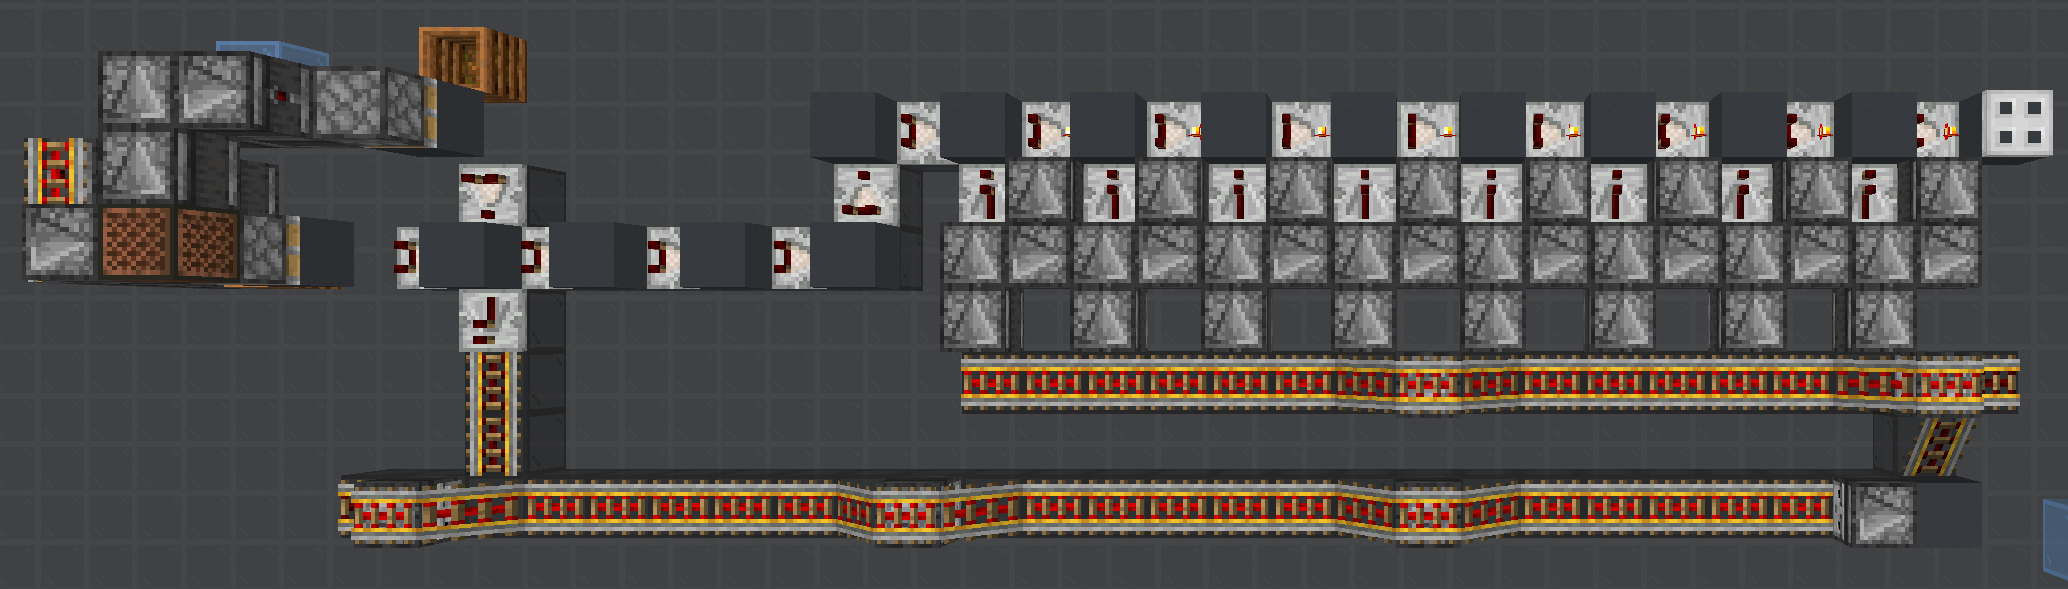
\includegraphics[width=0.48\textwidth]{redcmd.png}
    \caption{\centering 6gt-able Instant Comparator Wire}
\end{figure}

% For wide tables, a single column layout is better. It can be switched
% page-by-page.
\onecolumn

\section{Device Specifications}

\begin{table}[h]
    \caption{Device Specifications}
    \begin{tabularx}{\textwidth}{l | c c c | c | X}
        \thickhline
        \textbf{Parameter} & \textbf{Min.} & \textbf{Typ.} & \textbf{Max.} &
        \textbf{Unit} & \textbf{Conditions} \\
        \hline
        Throughput  & 6 & - & - & gt & Normal Usage \\
        \hline
        MC Version & 1.12 & 1.17.1 & - & MCV & Latest version at time of writing: 1.19.3\\
        \hline
        Dimensions & & 8 x 5 x 29 & & Blocks & \\
        \thickhline
\end{tabularx}
\end{table}

\section{Testing Data}
\begin{table}[h]
\caption{Executed Tests}
\begin{tabularx}{\textwidth}{l | X}
    \thickhline
    \textbf{Test} & \textbf{Result} \\
    \hline
    Throughput test & Device was able to function with 6gt clocked input. \\
    \thickhline
\end{tabularx}
\end{table}

\section{Download Information}
\begin{table}[h]
    \caption{Download Information}
    \begin{tabularx}{\textwidth}{l | l | l | X}
        \thickhline
        \textbf{Identifier} & \textbf{MC} & \textbf{File} & \textbf{Description} \\
        \hline
        WI01 & 1.17.1 & \href{https://github.com/Soontech-Annals/Archive/blob/8413f90a054b6c415703bae02badeba7541344f6/Archive/wiring/WI01\%206gt-able\%20Instant\%20Comparator\%20Wire/WI01\_6gt-able\_Instant\_Comparator\_Wire.litematic?raw=1}{WI01\_6gt-able\_Instant\_Comparator\_Wire.litematic} & Schematic of device. \\
        \hline
        \thickhline
    \end{tabularx}
\end{table}

\end{document}

